\documentclass[11pt]{article}
\usepackage{amssymb}
\usepackage{tikz}
\usepackage{fancyhdr}
\usepackage{extramarks}
\usepackage{pgfplots}
\usetikzlibrary{automata,positioning}
\usetikzlibrary{shapes.geometric, arrows}


\setlength{\topmargin}{-1.5in}
\setlength{\textheight}{9.5in}
\setlength{\oddsidemargin}{.125in}
\setlength{\textwidth}{6.25in}

\tikzstyle{startstop} = [rectangle, rounded corners, minimum width=3cm, minimum height=1cm,text centered, text width=3cm, draw=black, fill=red!30]
\tikzstyle{basicblock} = [rectangle, minimum width=3cm, minimum height=1cm,text centered, text width=3cm, draw=black, fill=blue!30]

\tikzstyle{io} = [trapezium, trapezium left angle=70, trapezium right angle=110, minimum width=3cm, minimum height=1cm, text centered, text width=2cm,draw=black, fill=blue!30]
\tikzstyle{process} = [rectangle, minimum width=3cm, minimum height=1cm, text centered, text width=2cm,draw=black, fill=orange!30]
\tikzstyle{decision} = [diamond, minimum width=3cm, minimum height=1cm, text centered, text width=2cm, draw=black, fill=green!30]



\tikzstyle{arrow} = [thick,->,>=stealth]
\begin{document}
	\title{
		\textbf{Car Logic Implementation}
	}
	\date{}
	\maketitle

	\begin{tikzpicture}[node distance=2.5cm]



	\node (hardware)[basicblock] {1 Hardware sensors};

	\node (autoDriver) [basicblock, below of=hardware] {2 Autonomous driver};

	\node (manAgent) [basicblock, below of=autoDriver] {6 Manufacturer agent};

	\node (carLogicAPI)[io, below of=manAgent, xshift=3cm]{5 Car Logic API};

	\node(meshAPI)[io, above of=carLogicAPI, xshift=3cm]{4 Mesh \\ API};

	\node(netHardware)[basicblock, above of=meshAPI] {3 Network hardware};



	\draw [arrow] (hardware.250) -- (autoDriver.110);
	\draw [arrow] (autoDriver.70) -- (hardware.290);

	\draw [arrow] (autoDriver.250) -- (manAgent.110);
	\draw [arrow] (manAgent.70) -- (autoDriver.290);

	\draw [arrow] (netHardware.250) -- (meshAPI.110);
	\draw [arrow] (meshAPI.70) -- (netHardware.290);

	\draw [arrow] (meshAPI.250) |- (carLogicAPI.10);
	\draw [arrow] (carLogicAPI.350) -| (meshAPI.290);

	\draw [arrow] (manAgent.290) |- (carLogicAPI.170);
	\draw [arrow] (carLogicAPI.190) -| (manAgent.250);

	\end{tikzpicture}

	\begin{enumerate}
		\item Hardware sensors: These are various data collection tools installed
			on the car, like compass, cameras, lidar and sonic sensors, accelerometers,
			and any other "raw" input signal.
		\item Autonomous driver: This manufacturer specific implementation
			is the interpretation of the raw input into abstract descriptions,
			such as lane position, position of other cars, and current direction
			and route. Also in this block would be the code to control the car,
			such as how to maintain a lane, how to set a speed, how to shift a lane.
			Also it should have saftey checks, like preventing collisions, avoiding
			objects, and limiting turning speed.
		\item Network hardware: This equipment allows for the transmition and
			reception of packets on some radio signal range. Targets include other
			cars, but also inteligent installations such as "caches" of accumulated
			data, traffic signals, repeaters, or smart road sections.
		\item Mesh API: This software allows the cars to form a mesh network, so that
			messages from any car can get to any other car in the mesh network. Most
			of the uses will be to transmit to cars immediately around the source, so
			a multitute of jumps would be rare.
		\item Car Logic API: The goal of this project. The idea here is to create a
			shared library that all manufacturers can implement how they choose, and
			so that the maximum colaberation can be had from cars on the road, whether
			or not they are the same model, manufacturer, or even whether or not they
			are smart cars. The goal here is to make it standard, and modular, so that
			the choice of how to implement and how much to implement, is left up to
			the manufactuter, that way they can make luxury models, budget models,
			improve, expand, and all while still being able to communicate with other
			cars on the road.
		\item Manufacturer implemenation: This would be the very last part of this
			stack to be developed. It would be the client of all other blocks in the
			diagram. This is where the creativity of the manufacturer shines.
			Car Logic API provides the manufacturer the toolset and standardization
			to do what they couldn't do before, to create a car that can collaborate
			with other manufacturer's cars.
	\end{enumerate}
\end{document}
